\documentclass[11pt]{article}

\newcommand{\extraauthor}{Daniele Bellavista\\
Scuola di Ingegneria ed Archiettura\\
Ingegneria Informatica Magistrale\\
Corso Sistemi Multiagente LM\\
}
\newcommand{\xauth}{Daniele Bellavista}
\newcommand{\xtitle}{Hovering Information: implementation using MAS}

\usepackage{amsmath}
\usepackage{placeins}
\usepackage{float}
\usepackage{ifpdf,ifluatex}
\ifluatex
\usepackage{fontspec}
\else
\usepackage[utf8x]{inputenc}
\fi

\usepackage{url}
\ifpdf
\usepackage{hyperref}
\hypersetup{unicode=true,
    pdftitle={\xtitle},
    pdfauthor={\xauth},
}
\fi

\usepackage{chngcntr}
\counterwithin{figure}{subsection}
\counterwithin{table}{subsection}

\usepackage{xspace}
\usepackage[usenames,dvipsnames]{xcolor}
\usepackage{graphicx}

\usepackage{listings}
\lstset{%
  breakatwhitespace=false,
  breaklines=true,
  captionpos=t,
  extendedchars=true,
  literate= {à}{{\`a}}1
            {η}{{$\eta$}}1
            {μ}{{$\mu$}}1
            {ρ}{{$\rho$}}1,
  frame=single,
  keepspaces=true,
  basicstyle=\ttfamily\footnotesize,
  keywordstyle=\color{blue},
  commentstyle=\color{OliveGreen},
  stringstyle=\color{RedOrange},
  numbers=left,
  numberstyle=\tiny\color{CadetBlue},
  rulecolor=\color{black},
  showspaces=false,
  showstringspaces=false,
  showtabs=false,
  tabsize=2,
  title=\lstname
}

\newcommand{\action}[1]{\texttt{#1}\xspace}
\newcommand{\code}[1]{{\small{\texttt{#1}}}\xspace}
\newcommand{\codescript}[1]{{\scriptsize{\texttt{#1}}}\xspace}

\begin{document}
\title{\xtitle}
\author{\xauth}

\maketitle

\section{Work Plan}
	\begin{enumerate}
		\item Capire Hoovering Information
  	\item Agente Smartphone
  	\item Agente Information
  	\item Agente Persona
  	\item Punti di interesse statici (espandibile a dinamici)
			\begin{enumerate}
				\item Modello spaziale
				\item Dinamica delle persone (gradiente, stigmergia, naive)
			\end{enumerate}
  	\item Simulatore
			\begin{enumerate}
				\item Grafica
				\item Raccolta dati
			\end{enumerate}
  	\item Punti di interesse dinamici
	\end{enumerate}

\section{Introduction}
	No central server, powerful hi-tech peers.

\section{Hovering Information and Social System analysis and design}
\label{sec:design}

The system should implement the hovering information system working inside
a social environment. Mobile nodes are owned by people, who move inside an
environment composed by anchors, that is locations where pieces of hovering
information are present. Anchors are usually bound to points of interest, but
in a more general way hovering information can be dynamically created by people.

The system should simulate an hovering information usage, inside an
environment.  People, carrying mobile nodes, have to walk with different
behaviour, emulating movements inside an area composed by points of interest.
The simulation should gather periodic data about hovering information status
and properties (i.e.\ availability, survivability and accessibility), nodes
position and communications link.

\subsection{Preliminary analysis}

Requirements implicate that the system is composed by three sub-systems:
\begin{enumerate}
	\item Simulator (graphic interface and data analyzer).
	\item Hovering information (composed by pieces of hovering information and
		mobile nodes).
	\item Social system (a group of hovering information users moving into
		the environment).
\end{enumerate}

Aside from required interfaces, these subsystems can be designed independently
from each other and each of them as different users. A simulator user may want
to create people and assign a behaviour, nodes and initial hovering information.
The simulator itself is the user of the social system and a single person inside
the latter system is an user of the hovering information service.

Social system requires people to move with different behaviours; a possible
solution is to assign \emph{social roles} with different behavior pattern.
Taking the cue from \cite{human} some roles can be defined:

\begin{description}
	\item[Guard:] a person who walks following a predefined path.
	\item[Employee:] a person who resides -works- near a certain point of interest.
	\item[Ant:] a person who performs a random walk but he's influenced in a
		certain manner by other people.
	\item[Group:] some people walking together, using one of the previous
		behaviour.
\end{description}

\subsection{Requirements Analysis}

From the requirements and the preliminary analysis considerations, the
\emph{SODA} process focuses on analysis and design of the \emph{Hovering
information system} and the \emph{Social system}, treating them as a single
system. The subsystem \emph{Simulator} doesn't require independent control or
intelligence, so the simulator interface can be assumed as a \emph{Legacy
System}, already present in the environment.

\subsubsection{Requirements Tables}

\begin{table}[H]
	\centering
	\begin{tabular}{|p{4cm}|p{8cm}|}
			\hline
			\textbf{Actor} & \textbf{Description} \\
			\hline
      Simulation Manager & The simulation manager, which renders the world and
      analyze its data. \\
			\hline
			Person & User of a mobile node. \\
			\hline
			Mobile node & Hovering information low-level user: discover, access and
			create the infrastructure for the pieces of hovering information. \\
			\hline
			Piece of Hovering Information & Hovering information instance. \\
			\hline
		\end{tabular}
	\caption{Actor table $(C)Ac_t$}
	\label{tab:cact}
\end{table}

\begin{table}[H]
	\centering
	\begin{tabular}{|p{4cm}|p{8cm}|}
			\hline
			\textbf{Requirement} & \textbf{Description} \\
			\hline
      Access Hovering Information & Access the hovering information
      available in the current position. \\
			\hline
			Create Hovering Information & Create a new hovering information. \\
			\hline
			Manage Device & Manage the mobile node resources such as storage,
			positioning and communication.  \\
			\hline
			Analyze Simulation & Analyze the system while the simulation is running.
			\\
			\hline
			Show Simulation & Show the simulation. \\
			\hline
			Move & Move within the social environment. \\
			\hline
			Survive & Stay alive. \\
			\hline
			Be available & Be available inside the anchor area. \\
			\hline
			Maintain accessibility & Cover the maximum possible area inside the
			anchor area. \\
			\hline
		\end{tabular}
	\caption{Requirement table $(C)Re_t$}
	\label{tab:cact}
\end{table}

\begin{table}[H]
	\centering
	\begin{tabular}{|p{4cm}|p{8cm}|}
			\hline
			\textbf{Actor} & \textbf{Requirement} \\
			\hline
			Person & Access Hovering Information, Create Hovering Information, Move. \\
			\hline
			Simulation Manager & Analyze Simulation, Show Simulation. \\
			\hline
			Mobile node & Access Hovering Information, Create Hovering Information, Manage Device. \\
			\hline
			Piece of Hovering Information & Access Hovering Information, Create Hovering Information,
			Survive, Be available, Maintain accessibility. \\
			\hline
		\end{tabular}
	\caption{Actor-Requirement table $(C)AR_t$}
	\label{tab:cart}
\end{table}

\subsubsection{Domain Tables}

\begin{table}[H]
	\centering
	\begin{tabular}{|p{4cm}|p{8cm}|}
			\hline
			\textbf{External Environment} & \textbf{Legacy system} \\
			\hline
			External & Simulator UI. \\
			\hline
		\end{tabular}
	\caption{External Environment-Legacy System table $(C)EELS_t$}
	\label{tab:ceelst}
\end{table}

\begin{table}[H]
	\centering
	\begin{tabular}{|p{4cm}|p{8cm}|}
			\hline
			\textbf{Legacy System} & \textbf{Description} \\
			\hline
			Simulator UI & Simulation output interface that shows simulation data. \\
			\hline
		\end{tabular}
	\caption{Legacy System table $(C)LS_t$}
	\label{tab:clst}
\end{table}

\subsubsection{Relations Tables}

\begin{table}[H]
	\centering
	\begin{tabular}{|p{4cm}|p{8cm}|}
			\hline
			\textbf{Relation} & \textbf{Description} \\
			\hline
			GUI & The system should send the information needed by the GUI. \\
			\hline
			Node Resources & High Level operations may require or depend from
			low-level node resources. \\
			\hline
			Node Interface & A person needs a node interface in order to use it for
			accessing or creating information. \\
			\hline
		\end{tabular}
	\caption{Relation table $(C)Rel_t$}
	\label{tab:crelt}
\end{table}

\begin{table}[H]
	\centering
	\begin{tabular}{|p{4cm}|p{8cm}|}
			\hline
			\textbf{Requirement} & \textbf{Relation} \\
			\hline
			Access Hovering Information & Node Resources, Node Interface.  \\
			\hline
			Create Hovering Information & Node Resources, Node Interface.  \\
			\hline
			Manage Device & Node Resources, Node Interface.  \\
			\hline
			Survive & Node Resources. \\
			\hline
			Be available & Node Resources. \\
			\hline
			Maintain accessibility & Node Resources. \\
			\hline
			Move & Living Space Respect. \\
			\hline
			Show Simulation & GUI. \\
			\hline
		\end{tabular}
	\caption{Requirement-Relation table $(C)RR_t$}
	\label{tab:crrt}
\end{table}

\begin{table}[H]
	\centering
	\begin{tabular}{|p{4cm}|p{8cm}|}
			\hline
			\textbf{Legacy-System} & \textbf{Relation} \\
			\hline
			Simulator UI & GUI. \\
			\hline
		\end{tabular}
	\caption{Relation-LegacySystem table $(C)RLS_t$}
	\label{tab:crlst}
\end{table}


\subsection{Analysis}

\subsubsection{References Tables}

\begin{table}[H]
	\centering
	\begin{tabular}{|p{4cm}|p{8cm}|}
			\hline
			\textbf{Requirement} & \textbf{Task} \\
			\hline
			Access Hovering Information & access\_information \\
			\hline
			Create Hovering Information & create\_information \\
			\hline
			Analyze Simulation & analyze\_simulation, inquire\_world \\
			\hline
			Show Simulation & show\_simulation \\
			\hline
			Survive & survive\_task \\
			\hline
			Be available & be\_available\_task \\
			\hline
			Maintain accessibility & maintain\_accessibility\_task\\
			\hline
			Move & move\_task \\
			\hline
		\end{tabular}
	\caption{Reference Requirement-Task table $(C)RRT_t$}
	\label{tab:crrtt}
\end{table}

\begin{table}[H]
	\centering
	\begin{tabular}{|p{4cm}|p{8cm}|}
			\hline
			\textbf{Requirement} & \textbf{Function} \\
			\hline
			Manage Device & get\_position, discover\_neighbours, communicate, manage\_storage \\
			\hline
		\end{tabular}
	\caption{Reference Requirement-Function table $(C)RRF_t$}
	\label{tab:crrft}
\end{table}

\begin{table}[H]
	\centering
	\begin{tabular}{|p{4cm}|p{8cm}|}
			\hline
			\textbf{Requirement} & \textbf{Topology} \\
			\hline
			Access Hovering Information & Anchor Area, Communication Range, Node Topology. \\
			\hline
			Create Hovering Information & Anchor Area, Communication Range, Node Topology. \\
			\hline
			Manage Device & Communication Range, Node Topology. \\
			\hline
			Hover & Anchor Area, Communication Range, Node Topology. \\
			\hline
			Show Simulation & World. \\
			\hline
			Analyze Simulation & World. \\
			\hline
			Move & World. \\
			\hline
		\end{tabular}
	\caption{Reference Requirement-Topology table $(C)RRTo_t$}
	\label{tab:crrtot}
\end{table}

\begin{table}[H]
	\centering
	\begin{tabular}{|p{4cm}|p{8cm}|}
			\hline
			\textbf{Requirement} & \textbf{Dependency} \\
			\hline
			 & \\
			\hline
		\end{tabular}
		\caption{Reference Requirement-Dependency table $(C)RReqD_t$}
	\label{tab:crreqdt}
\end{table}

\begin{table}[H]
	\centering
	\begin{tabular}{|p{4cm}|p{8cm}|}
			\hline
			\textbf{Legacy System} & \textbf{Function} \\
			\hline
			Simulator UI & render. \\
			\hline
		\end{tabular}
	\caption{Reference Legacy System-Function table $(C)RLSF_t$}
	\label{tab:crlsft}
\end{table}

\begin{table}[H]
	\centering
	\begin{tabular}{|p{4cm}|p{8cm}|}
			\hline
			\textbf{Legacy System} & \textbf{Topology} \\
			\hline
			Simulator UI & World. \\
			\hline
		\end{tabular}
	\caption{Reference Legacy System-Topology table $(C)RLST_t$}
	\label{tab:crlsTt}
\end{table}

\begin{table}[H]
	\centering
	\begin{tabular}{|p{4cm}|p{8cm}|}
			\hline
			\textbf{Relation} & \textbf{Dependency} \\
			\hline
			GUI & GUIDep \\
			\hline
			Node Resources & NeighbourDep, StorageDep, PositionDep. \\
			\hline
			Node Interface & NodeIfDep. \\
			\hline
		\end{tabular}
	\caption{Reference Relation-Dependency table $(C)RRD_t$}
	\label{tab:crrdt}
\end{table}

\subsubsection{Responsibilities Tables}

\begin{table}[H]
	\centering
	\begin{tabular}{|p{5cm}|p{7cm}|}
			\hline
			\textbf{Task} & \textbf{Description} \\
			\hline
			access\_information & Access the needed information available in the
			current position.\\
			\hline
			create\_information & Create a new hovering information. \\
			\hline
			analyze\_simulation & Analyze the simulation.\\
			\hline
			inquire\_world & Get the data needed by the analysis process.  \\
			\hline
			show\_simulation & Create a displayable representation of the world. \\
			\hline
			move\_task & Move with a certain behaviour inside the environment. \\
			\hline
			survive & Jumps or replicates to mobile nodes in order to keep an high
			survivability. \\
			\hline
			be\_available & Jumps or replicates to mobile nodes in order to keep an
			high availability. \\
			\hline
			maintain\_accessibility & Jumps or replicates to mobile nodes in order to
			keep an high accessibility. \\
			\hline
		\end{tabular}
	\caption{Task table $(C)T_t$}
	\label{tab:ctt}
\end{table}

\begin{table}[H]
	\centering
	\begin{tabular}{|p{5cm}|p{7cm}|}
			\hline
			\textbf{Function} & \textbf{Description} \\
			\hline
			render & Show a graphical representation of the simulated system. \\
			\hline
			get\_position & Return the position of a mobile node. \\
			\hline
			discover\_neighbours & Discover the neighbours of a mobile nodes. \\
			\hline
			communicate & Send a message to a mobile node. \\
			\hline
			manage\_storage & Manage mobile node storage resource. \\
			\hline
		\end{tabular}
	\caption{Function table $(C)F_t$}
	\label{tab:cft}
\end{table}

\subsubsection{Topologies Tables}

\begin{table}[H]
	\centering
	\begin{tabular}{|p{4cm}|p{8cm}|}
			\hline
			\textbf{Topology} & \textbf{Description} \\
			\hline
			Node Topology & The mobile node, positioned inside the world, seen
			as a topological constraint. \\
			\hline
			Anchor Area & Area associated to each hovering information, defined as a
			circular area with center into the \emph{anchor location} and radius the
			\emph{anchor radius}.\\
			\hline
			Communication Range & The maximum effective distance of a \emph{p2p}
			mobile node communication. \\
			\hline
			World & The environment. \\
			\hline
		\end{tabular}
	\caption{Topology table $(C)Top_t$}
	\label{tab:ctopt}
\end{table}

\begin{table}[H]
	\centering
	\begin{tabular}{|p{4cm}|p{8cm}|}
			\hline
			\textbf{Task} & \textbf{Topology} \\
			\hline
			access\_information& Node Topology, Anchor Area, Communication Range, World.\\
			\hline
			create\_information & Node Topology, Anchor Area, Communication Range, World.\\
			\hline
			survive & Anchor Area, Communication Range, World. \\
			\hline
			be\_available & Anchor Area, Communication Range, World. \\
			\hline
			maintain\_accessibility & Anchor Area, Communication Range, World. \\
			\hline
			world\_task & World. \\
			\hline
			show\_simulation & World. \\
			\hline
		\end{tabular}
		\caption{Task-Topology table $(C)TTop_t$}
	\label{tab:cttopt}
\end{table}

\begin{table}[H]
	\centering
	\begin{tabular}{|p{4cm}|p{8cm}|}
			\hline
			\textbf{Function} & \textbf{Topology} \\
			\hline
			render & World.\\
			\hline
			inquire\_world & World.\\
			\hline
			discover\_neighbour & Communication Range, World, Node Topology. \\
			\hline
			communicate & Communication Range, World, Node Topology. \\
			\hline
			get\_position & World, Node Topology. \\
			\hline
			manage\_storage & Node Topology. \\
			\hline
		\end{tabular}
	\caption{Function-Topology table $(C)FTop_t$}
	\label{tab:cftopt}
\end{table}


\subsubsection{Dependency Tables}

\begin{table}[H]
	\centering
	\begin{tabular}{|p{4cm}|p{8cm}|}
			\hline
			\textbf{Dependency} & \textbf{Description} \\
			\hline
			GUIDep & Make data available for GUI purposes. \\
			\hline
			NeighbourDep & A mobile node is a neighbour of another if both are in
			communication range. \\
			\hline
			StorageDep & High level operations depends on mobile node storage availability. \\
			\hline
			%NodeUIDep & A mobile node should show information about the hovering
			%system on the mobile UI. \\
			%\hline
			NodeIfDep & A person needs a node interface in order to use it for access
			or creating hovering information. \\
			\hline
			InquireDep & Get system information for analysis purposes. \\
			\hline
			BoundedWorldDep & A person cannot move outside the world. \\
			\hline
		\end{tabular}
	\caption{Dependency table $(C)D_t$}
	\label{tab:cdt}
\end{table}

\begin{table}[H]
	\centering
	\begin{tabular}{|p{5cm}|p{7cm}|}
			\hline
			\textbf{Task} & \textbf{Dependency} \\
			\hline
			access\_information & CommDep, PositionDep, NodeIfDep. \\
			\hline
			create\_information & CommDep, PositionDep, StorageDep, NodeIfDep. \\
			\hline
			survive\_task & NeighbourDep, PositionDep, StorageDep. \\
			\hline
			be\_available\_task &  NeighbourDep, PositionDep, StorageDep. \\
			\hline
			maintain\_accessibility\_task & CommDep, PositionDep, StorageDep. \\
			\hline
			move\_task & LivingSpaceDep, BoundedWorldDep. \\
			\hline
			show\_simulation & GUIDep. \\
			\hline
			analyze\_simulation & InquireDep. \\
			\hline
			inquire\_world & InquireDep. \\
			\hline
		\end{tabular}
	\caption{Task-Dependency table $(C)TD_t$}
	\label{tab:ctdt}
\end{table}

\begin{table}[H]
	\centering
	\begin{tabular}{|p{5cm}|p{7cm}|}
			\hline
			\textbf{Function} & \textbf{Dependency} \\
			\hline
			render & GUIDep. \\
			\hline
			discover\_neighbours & NeighbourDep. \\
			\hline
			communicate & NeighbourDep. \\
			\hline
			manage\_storage & StorageDep. \\
			\hline
			get\_position & PositionDep. \\
			\hline
		\end{tabular}
	\caption{Function-Dependency table $(C)FD_t$}
	\label{tab:cfdt}
\end{table}

\begin{table}[H]
	\centering
	\begin{tabular}{|p{4cm}|p{8cm}|}
			\hline
			\textbf{Topology} & \textbf{Dependency} \\
			\hline
			Node Topology & StorageDep, PositionDep, NodeIfDep, NeighbourDep. \\
			\hline
			Anchor Area & SimDataDep, PositionDep.\\
			\hline
			Communication Range & SimDataDep, NeighbourDep. \\
			\hline
			World & InquireDep, GUIDep, BoundedWorldDep. \\
			\hline
		\end{tabular}
	\caption{Topology-Dependency table $(C)TopD_t$}
	\label{tab:ctopdt}
\end{table}

\subsection{Architectural Design}

Communication mechanisms were not specified during analysis, so, in order to
reduce design and implementation complexity, I assume that the only way to
communicate is by \emph{dispatches}, that is asynchronous message passing with
strong expectation by the sender that the receiver will process the message.

The communication act is then decomposed into two primitives: \emph{in} and
\emph{out}. The communication resource is shared, so each user must have an
unique id.

\subsubsection{Transition Tables}

\begin{table}[H]
	\centering
	\begin{tabular}{|p{4cm}|p{8cm}|}
			\hline
			\textbf{Role} & \textbf{Task} \\
			\hline
      Simulation Manager & analyze\_simulation, inquire\_world, show\_simulation.   \\
			\hline
			Person & access\_information, create\_information, move\_task \\
			\hline
			Mobile node & access\_information, create\_information.  \\
			\hline
			Piece of Hovering Information & survive\_task, be\_available\_task,
			maintain\_accessibility\_task. \\
			\hline
		\end{tabular}
	\caption{Transition Role-Task table $(C)TRT_t$}
	\label{tab:ctrtt}
\end{table}

\begin{table}[H]
	\centering
	\begin{tabular}{|p{4cm}|p{8cm}|}
			\hline
			\textbf{Task} & \textbf{Action} \\
			\hline
			analyze\_simulation & AnalyzeSimulation. \\
			\hline
			inquire\_world & InquireNodes, InquireHoveringInformations, InquireEnvironment. \\
			\hline
			show\_simulation & ShowSimulation. \\
			\hline
			access\_information & AccessInformation, ListInformation, ShowInformationToUI,
			AccessInformationData.\\
			\hline
			create\_information & CreateInformation, CreateViaUI. \\
			\hline
			move\_task & SenseAction, MoveAction. \\
			\hline
			survive\_task & Jump, Replicate. \\
			\hline
			be\_available\_task & Jump, Replicate. \\
			\hline
			maintain\_accessibility\_task & Jump, Replicate. \\
			\hline
		\end{tabular}
	\caption{Transition Task-Action table $(C)TTA_t$}
	\label{tab:cttat}
\end{table}

\begin{table}[H]
	\centering
	\begin{tabular}{|p{4cm}|p{8cm}|}
			\hline
			\textbf{Resource} & \textbf{Function} \\
			\hline
			SimulatorUIRes & render. \\
			\hline
			MobileResource & discover\_neighbour, get\_position, manage\_ui,
			manage\_storage. \\
			\hline
		\end{tabular}
	\caption{Transition Resource-Function table $(C)TRF_t$}
	\label{tab:ctrft}
\end{table}

\begin{table}[H]
	\centering
	\begin{tabular}{|p{4cm}|p{8cm}|}
			\hline
			\textbf{Function} & \textbf{Operation} \\
			\hline
			render & RenderWorld. \\
			\hline
			manage\_storage & InsertData, RemoveData, GetRemainingSpace,
			GetMaximumSize. \\
			\hline
			discover\_neighbour & DiscoveNeighbour. \\
			\hline
			Communicate & SendMessage, ReceiveMessage. \\
			\hline
			get\_position & ObtainPosition. \\
			\hline
		\end{tabular}
	\caption{Transition Function-Operation table $(C)TFO_t$}
	\label{tab:ctfot}
\end{table}

\begin{table}[H]
	\centering
	\begin{tabular}{|p{4cm}|p{8cm}|}
			\hline
			\textbf{Dependency} & \textbf{Interaction} \\
			\hline
			GUIDep & Render Interaction \\
			\hline
      NeighbourDep & DiscoverNeighbour Interaction, SendMessage Interaction,
      ReceiveMessage Interaction \\
			\hline
			StorageDep & InsertNewPiece Interaction, RemovePiece Interaction \\
			\hline
			NodeIfDep & User Create Interaction, ShowInformation Interaction \\
			\hline
			InquireDep & Inquisition Interaction\\
			\hline
			BoundedWorldDep & \\
			\hline
		\end{tabular}
	\caption{Transition Dependency-Interaction table $(C)TDI_t$}
	\label{tab:ctdit}
\end{table}

\begin{table}[H]
	\centering
	\begin{tabular}{|p{4cm}|p{8cm}|}
			\hline
			\textbf{Dependency} & \textbf{Rule} \\
			\hline
			NeighbourDep & Neighbour Rule, Send Rule, Receive Rule\\
			\hline
			StorageDep & Storage Rule \\
			\hline
			NodeIfDep & \\
			\hline
			InquireDep & \\
			\hline
			BoundedWorldDep & Bounded World Rule\\
			\hline
		\end{tabular}
	\caption{Transition Dependency-Rule table $(C)TDRu_t$}
	\label{tab:ctdrut}
\end{table}

\begin{table}[H]
	\centering
	\begin{tabular}{|p{4cm}|p{8cm}|}
			\hline
			\textbf{Topology} & \textbf{Space} \\
			\hline
			Anchor Area & Anchor Area Space.\\
			\hline
			Communication Range & Communication Range Space. \\
			\hline
			World & World Space. \\
			\hline
			Node Topology & Node Space. \\
			\hline
		\end{tabular}
	\caption{Transition Topology-Space table $(C)TTopS_t$}
	\label{tab:cttopst}
\end{table}

\subsubsection{Entities Tables}

\begin{table}[H]
	\centering
	\begin{tabular}{|p{5cm}|p{7cm}|}
			\hline
			\textbf{Action} & \textbf{Description} \\
			\hline
			AccessInformation & Find and access to the data of the required
			information. \\
			\hline
			ListInformation & Gets all the information available to the mobile node
			that is valid in the current position.\\
			\hline
			CreateInformation & Create a new hovering information. \\
			\hline
			CreateViaUI & A mobile user can create an hovering information using the
			mobile UI. \\
			\hline
      ShowInformationToUI & Show available information to the device UI, so
      that it's accessible from the user.\\
			\hline
			Replicate & Make a copy of the hovering information to be transferred to
			another mobile node. \\
			\hline
			Jump & Transfer the hovering information to another mobile node. \\
			\hline
			AccessInformationData & Allow access to the hovering information data. \\
			\hline
			SenseAction & Obtain the near person or points of interest. \\
			\hline
			MoveAction & Basic movement in the environment. \\
      \hline
      AnalyzeSimulation & Analyze the system properties such as hovering
      information requirements and complex network parameters. \\
			\hline
			ShowSimulation & Obatin a renderable world representation. \\
			\hline
			InquireNodes & Get all the information about mobile nodes.\\
			\hline
			InquireHoveringInformation & Get all the information about pieces of
			hovering information.\\
			\hline
			InquireEnvironment & Get extra information about environment.\\
			\hline
		\end{tabular}
	\caption{Action table $(C)A_t$}
	\label{tab:cat}
\end{table}

\begin{table}[H]
	\centering
	\begin{tabular}{|p{4cm}|p{8cm}|}
			\hline
			\textbf{Operation} & \textbf{Description} \\
			\hline
			RenderWorld & Render a representation of the world. \\
			\hline
			DiscoveNeighbour & Discover peers node inside the communication range. \\
			\hline
      SendMessage & Send an asynchronous message to a node that resides in
      communication range. \\
			\hline
      ReceiveMessage & Receive a message. Blocks if there are no messages. \\
			\hline
			InsertData & Insert a data into the mobile node buffer. \\
			\hline
			RemoveData & Remove a data from the mobile node buffer. \\
			\hline
			GetRemainingSpace & Obtain the space left of the mobile node buffer. \\
			\hline
			GetMaximumSize & Obtain the total space of the mobile node buffer. \\
			\hline
			ObtainPosition & Obtain the current node position using some location
			device. \\
			\hline
		\end{tabular}
	\caption{Operation table $(C)O_t$}
	\label{tab:cot}
\end{table}

\begin{table}[H]
	\centering
	\begin{tabular}{|p{4cm}|p{8cm}|}
			\hline
			\textbf{Role} & \textbf{Action} \\
			\hline
			Simulation Manager & AnalyzeSimulation, InquireNodes, InquireHoveringInformations, In-
			quireEnvironment, ShowSimulation. \\
			\hline
			Person & SenseAction, MoveAction, CreateViaUI. \\
			\hline
			Mobile node & ManageDevice, ListInformation, CreateInformation, ShowInformationToUI.  \\
			\hline
			Piece of Hovering Information & Replicate, Jump, AccessInformationData. \\
			\hline
		\end{tabular}
	\caption{Role-Action table $(C)RA_t$}
	\label{tab:rat}
\end{table}

\begin{table}[H]
	\centering
	\begin{tabular}{|p{4cm}|p{8cm}|}
			\hline
			\textbf{Resource} & \textbf{Operation} \\
			\hline
			SimulatorUIRes & RenderWorld. \\
			\hline
			MobileResource & InsertData, RemoveData, GetRemainingSpace,
			GetMaximumSize, DiscoveNeighbour, SendMessage, ReceiveMessage, ObtainPosition. \\
			\hline
		\end{tabular}
	\caption{Resource-Operation table $(C)RO_t$}
	\label{tab:crot}
\end{table}

\subsubsection{Interactions Tables}

\begin{table}[H]
	\centering
	\begin{tabular}{|p{4cm}|p{8cm}|}
			\hline
			\textbf{Interaction (Social \& Simulation)} & \textbf{Description} \\
			\hline
			Sense Interaction & Sense the world, obtaining information about other
			people and points of interest. \\
			\hline
			Move Interaction & Move inside the world, following a certain behaviour.
			\\
			\hline
			User Create Interaction & Mobile users have to communicate with the
			mobile node in order to create information. \\
			\hline
			\hline
			Inquisition Interaction & World inquisition for simulation analysis and
			management purposes. \\
			\hline
			Render Interaction & The system should interact with the GUI. \\
			\hline
		\end{tabular}
	\caption{Interaction table $(C)Isa_t$}
	\label{tab:cisat}
\end{table}

\begin{table}[H]
	\centering
	\begin{tabular}{|p{4cm}|p{8cm}|}
			\hline
			\textbf{Interaction (Hovering System)} & \textbf{Description} \\
			\hline
			ShowInformation Interaction & Show the mobile user the available information. \\
			\hline
			InsertNewPiece Interaction & Insert if possible a new piece of hovering
			information inside a mobile node buffer. \\
			\hline
			RemovePiece Interaction & Remove a piece of hovering information from the
			hosting mobile node buffer. \\
			\hline
			Access Interaction & Mobile nodes have to communicate together in order to
			access an hovering information. \\
			\hline
			List Interaction & Mobile nodes have to communicate together in order to
			obtain the list of available hovering information. \\
			\hline
			DiscoverNeighbour Interaction & Mobile nodes or piece of hovering
			information have to know the neighbours. \\
			\hline
      SendMessage Interaction & Mobile nodes can send messages to their
      neighbour, specifying an high-level receiver. \\
			\hline
      ReceiveMessage Interaction & Mobile nodes can receive messages specifying
      an high-level receiver. \\
			\hline
			\hline
			AccessInformationData Interaction & Mobile nodes must interact with Pieces
			of Hovering Information in order to get their data. \\
			\hline
			Jump Interaction & Jump from a mobile node to another. \\
			\hline
			Replication Interaction & Replicate to another mobile node. \\
			\hline
		\end{tabular}
	\caption{Interaction table $(C)Ihov_t$}
	\label{tab:cihovt}
\end{table}

\begin{table}[H]
	\centering
	\begin{tabular}{|p{5cm}|p{7cm}|}
			\hline
			\textbf{Action} & \textbf{Interaction} \\
			\hline
			AccessInformation & Access Interaction, Communication Interaction. \\
			\hline
			ListInformation & List Interaction, Communication Interaction. \\
			\hline
			CreateInformation & Communication Interaction, Communication Interaction.\\
			\hline
			CreateViaUI & User Create Interaction \\
			\hline
      ShowInformationToUI & ShowInformation Interaction.\\
			\hline
			Replicate & Replication Interaction, Communication Interaction.  \\
			\hline
			Jump & Jump Interaction, Communication Interaction. \\
			\hline
			AccessInformationData & AccessInformationData Interaction \\
			\hline
			MoveAction & Move Interaction \\
			\hline
			SenseAction & Sense Interaction \\
			\hline
			AnalyzeSimulation & Inquisition Interaction \\
			\hline
			InquireNodes & Inquisition Interaction. \\
			\hline
			InquireHoveringInformation & Inquisition Interaction. \\
			\hline
			InquireEnvironment & Inquisition Interaction. \\
			\hline
			ShowSimulation & Render Interaction \\
			\hline
		\end{tabular}
	\caption{Action-Interaction table $(C)AcI_t$}
	\label{tab:cacit}
\end{table}

\begin{table}[H]
	\centering
	\begin{tabular}{|p{4cm}|p{8cm}|}
			\hline
			\textbf{Operation} & \textbf{Interaction} \\
			\hline
			RenderWorld & Render Interaction. \\
			\hline
			DiscoveNeighbour & DiscoverNeighbour Interaction. \\
			\hline
			SendMessage & SendMessage Interaction. \\
			\hline
			ReceiveMessage & ReceiveMessage Interaction. \\
			\hline
			InsertData & InsertNewPiece Interaction. \\
			\hline
			RemoveData &  RemovePiece Interaction. \\
			\hline
			GetRemainingSpace & InsertNewPiece Interaction, RemovePiece Interaction.  \\
			\hline
			GetMaximumSize & InsertNewPiece Interaction, RemovePiece Interaction.  \\
			\hline
			ObtainPosition & Jump Interaction, Replicate Interaction, List
			Interaction, Access Interaction.  \\
			\hline
		\end{tabular}
	\caption{Operation-Interaction table $(C)OpI_t$}
	\label{tab:opit}
\end{table}

\subsubsection{Constraints Tables}

\begin{table}[H]
	\centering
	\begin{tabular}{|p{4cm}|p{8cm}|}
			\hline
			\textbf{Rule} & \textbf{Description} \\
			\hline
			Accessible Rule & A mobile node can access an hovering information, if it
			resides in its anchor area. \\
			\hline
			Listing Rule & A mobile node answers to a listing interaction only with
			information accessible from the sender position. \\
			\hline
			Creation Rule & An hovering information can be created from a mobile node
			residing in the anchor area. \\
			\hline
			Storage Rule & A mobile node cannot store more information than its
			buffer permits. \\
			\hline
			Neighbour Rule & A mobile node is reachable (is a neighbour) from
			another if both are in communication range. \\
			\hline
			Movement Duplicate Rule & If a neighbour mobile node doesn't contain the same
			hovering information, movement or replication is allowed. \\
			\hline
			Bounded World Rule & People cannot move outside the world. \\
			\hline
			Node Location Rule & A mobile node and an hovering information can access
			only its own mobile resource. \\
			\hline
			Send Rule & A message can be delivered only to nodes in communication range. \\
			\hline
			Receive Rule & A message can be picked up only by the high-level receiver. \\
			\hline
		\end{tabular}
	\caption{Rule table $(C)Ru_t$}
	\label{tab:crut}
\end{table}

\begin{table}[H]
	\centering
	\begin{tabular}{|p{4cm}|p{8cm}|}
			\hline
			\textbf{Interaction} & \textbf{Rule} \\
			\hline
			Move Interaction & Bounded World Rule. \\
			\hline
			Sense Interaction & \\
			\hline
			ShowInformation Interaction & \\
			\hline
			InsertNewPiece Interaction & Storage Rule, Node Location Rule \\
			\hline
			Access Interaction & Accessible Rule, Neighbour Rule \\
			\hline
			List Interaction & Listing Rule, Neighbour Rule \\
			\hline
			AccessInformationData Interaction & Neighbour Rule\\
			\hline
			DiscoverNeighbour Interaction & Neighbour Rule\\
			\hline
			Send Interaction & Send Rule, Neighbour Rule\\
			\hline
			Receive Interaction & Receive Rule, Neighbour Rule\\
			\hline
			User Create Interaction & \\
			\hline
			User Access Interaction & \\
			\hline
			Jump Interaction & Movement Duplicate Rule, Neighbour Rule \\
			\hline
			Replication Interaction & Movement Duplicate Rule, Neighbour Rule \\
			\hline
			Render Interaction & \\
			\hline
			Inquisition Interaction & \\
			\hline
		\end{tabular}
	\caption{Interaction-Rule table $(C)IRu_t$}
	\label{tab:cirut}
\end{table}

\begin{table}[H]
	\centering
	\begin{tabular}{|p{4cm}|p{8cm}|}
			\hline
			\textbf{Resource} & \textbf{Rule} \\
			\hline
      MobileResource & Storage Rule, Neighbour Rule, Node Location Rule, Send
      Rule, Receive Rule. \\
			\hline
		\end{tabular}
	\caption{Resource-Rule table $(C)ReRu_t$}
	\label{tab:crerut}
\end{table}

\begin{table}[H]
	\centering
	\begin{tabular}{|p{4cm}|p{8cm}|}
			\hline
			\textbf{Role} & \textbf{Rule} \\
			\hline
			Simulation Manager & \\
			\hline
			Person & Bounded World Rule. \\
			\hline
			Piece of Hovering Information &  Movement Duplicate
			Rule, Storage Rule, Neighbour Rule, Send Rule, Receive Rule.  \\
			\hline
			Mobile Node & Accessible Rule, Listing Rule, Creation Rule, Neighbour
			Rule, Send Rule, Receive Rule, Node Location Rule. \\
			\hline
		\end{tabular}
	\caption{Role-Rule table $(C)RoRu_t$}
	\label{tab:crorut}
\end{table}

\begin{table}[H]
	\centering
	\begin{tabular}{|p{4cm}|p{8cm}|}
			\hline
			\textbf{Space} & \textbf{Rule} \\
			\hline
			Anchor Area Space & Accessible Rule, Listing Rule, Creation Rule. \\
			\hline
			Communication Range Space & Neighbour Rule, Send Rule, Receive Rule. \\
			\hline
			Node Space & Node Location Rule, Accessible Rule, Listing Rule, Creation Rule. \\
			\hline
			World Space & Bounded World Rule. \\
			\hline
		\end{tabular}
	\caption{Space-Rule table $(C)SRu_t$}
	\label{tab:cot}
\end{table}

\subsubsection{Topological Tables}

\begin{table}[H]
	\centering
	\begin{tabular}{|p{4cm}|p{8cm}|}
			\hline
			\textbf{Space} & \textbf{Description} \\
			\hline
			Node Space & Mobile node space: located in a specific position, holds a
			mobile resource. \\
			\hline
			Anchor Area Space & Area associated to each hovering information, defined as a
			circular area with center into the \emph{anchor location} and radius the
			\emph{anchor radius}.\\
			\hline
			Communication Range Space & The maximum effective distance of a \emph{p2p}
			mobile node communication. \\
			\hline
			World Space & The environment. \\
			\hline
		\end{tabular}
	\caption{Space table $(C)S_t$}
	\label{tab:st}
\end{table}

\begin{table}[H]
	\centering
	\begin{tabular}{|p{4cm}|p{8cm}|}
			\hline
			\textbf{Space} & \textbf{Connection} \\
			\hline
			Communication Range Space & Centered, Inside. \\
			\hline
			Node Space & Centered, Inside. \\
			\hline
			Anchor Area Space & Inside. \\
			\hline
			World Space & Inside. \\
			\hline
		\end{tabular}
	\caption{Space-Connection table $(C)SC_t$}
	\label{tab:sct}
\end{table}

\begin{table}[H]
	\centering
	\begin{tabular}{|p{4cm}|p{8cm}|}
			\hline
			\textbf{Resource} & \textbf{Space} \\
			\hline
			SimulatorUIRes & World Space \\
			\hline
			Node Resource & Node Space \\
			\hline
		\end{tabular}
	\caption{Resource-Space table $(C)ReS_t$}
	\label{tab:crest}
\end{table}

\begin{table}[H]
	\centering
	\begin{tabular}{|p{4cm}|p{8cm}|}
			\hline
			\textbf{Role} & \textbf{Space} \\
			\hline
			Simulation Manager & World Space. \\
			\hline
			Person & World Space, Anchor Space. \\
			\hline
			Mobile node & Node Space, Anchor Space. \\
			\hline
			Piece of Hovering Information & Anchor Space, Node Space. \\
			\hline
		\end{tabular}
	\caption{Role-Space table $(C)RoS_t$}
	\label{tab:cost}
\end{table}

\subsection{Detailed Design}

\subsubsection{Carving Diagram}


\subsubsection{Mapping Tables}

\begin{table}[H]
	\centering
	\begin{tabular}{|p{4cm}|p{8cm}|}
			\hline
			\textbf{Agent} & \textbf{Role} \\
			\hline
			Person & Person. \\
			\hline
			MobileNode & Mobile Node.  \\
			\hline
			Hovering & Piece of Hovering Information. \\
			\hline
			Simulator & Simulation Manager. \\
			\hline
		\end{tabular}
	\caption{Mapping Agent-Role table $(C)MAR_t$}
	\label{tab:cmart}
\end{table}

\begin{table}[H]
	\centering
	\begin{tabular}{|p{4cm}|p{8cm}|}
			\hline
			\textbf{Society} & \textbf{Role} \\
			\hline
			& \\
			\hline
		\end{tabular}
	\caption{Mapping Society-Role table $(C)MSR_t$}
	\label{tab:cmsrt}
\end{table}

\begin{table}[H]
	\centering
	\begin{tabular}{|p{4cm}|p{8cm}|}
			\hline
			\textbf{Artifact} & \textbf{Action} \\
			\hline
			Body Artifact & MoveAction, SenseAction. \\
			\hline
			MobileUI Artifact & CreateViaUI Action, ShowInformationToUI Action. \\
			\hline
			MobileUIInterface Artifact & ShowInformationToUI Action, CreateViaUI Action. \\
			\hline
      Simulator Artifact & ShowSimulation, AnalyzeSimulation,
      InquireNodes, InquireHoveringInformation, InquireEnvironment. \\
			\hline
			HoveringInformation Artifact & AccessInformationData. \\
			\hline
			MobileNode Artifact & CreateInformation \\
			\hline
		\end{tabular}
	\caption{Mapping Artifact-Action table $(C)MAAc_t$}
	\label{tab:cmaact}
\end{table}

\begin{table}[H]
	\centering
	\begin{tabular}{|p{4cm}|p{8cm}|}
			\hline
			\textbf{Artifact} & \textbf{Resource} \\
			\hline
			UI Artifact & SimulatorUIRes. \\
			\hline
			MobileResource Artifact & MobileResource. \\
			\hline
		\end{tabular}
	\caption{Mapping Artifact-Resource table $(C)MArR_t$}
	\label{tab:cmarrt}
\end{table}

\begin{table}[H]
	\centering
	\begin{tabular}{|p{4cm}|p{8cm}|}
			\hline
			\textbf{Aggregate} & \textbf{Resource} \\
			\hline
			& \\
			\hline
		\end{tabular}
	\caption{Mapping Aggregate-Resource table $(C)MAggR_t$}
	\label{tab:cmaggrt}
\end{table}

\begin{table}[H]
	\centering
	\begin{tabular}{|p{4cm}|p{8cm}|}
			\hline
			\textbf{Artifact} & \textbf{Operation} \\
			\hline
			UI Artifact & RenderWorld. \\
			\hline
      MobileResource Artifact & DiscoveNeighbour, SendMessage, ReceiveMessage,
      InsertData, RemoveData, GetRemainingSpace, GetMaximumSize,
      ObtainPosition. \\
			\hline
		\end{tabular}
	\caption{Mapping Artifact-Operation table $(C)MArOp_t$}
	\label{tab:cmaropt}
\end{table}

\begin{table}[H]
	\centering
	\begin{tabular}{|p{4cm}|p{8cm}|}
			\hline
			\textbf{Artifact} & \textbf{Rule} \\
			\hline
			Body Artifact & Bounded World Rule. \\
			\hline
			MobileResource Artifact & Storage Rule, Neighbour Rule, Node Location
			Rule, Movement Duplicate Rule. \\
			\hline
		\end{tabular}
	\caption{Mapping Artifact-Rule table $(C)MArRu_t$}
	\label{tab:cmarrut}
\end{table}

\begin{table}[H]
	\centering
	\begin{tabular}{|p{4cm}|p{8cm}|}
			\hline
			\textbf{Space} & \textbf{Workspace} \\
			\hline
			Node Space & Node Workspace. \\
			\hline
			Anchor Area Space & Anchor Area. \\
			\hline
			Communication Range Space & Communication Range.\\
			\hline
			World Space & World. \\
			\hline
		\end{tabular}
	\caption{Mapping Space-Workspace table $(C)MSW_t$}
	\label{tab:cmsrt}
\end{table}

\begin{table}[H]
	\centering
	\begin{tabular}{|p{4cm}|p{8cm}|}
			\hline
			\textbf{Interaction} & \textbf{Use} \\
			\hline
			Move Interaction & Move Use \\
			\hline
			Sense Interaction & Sense Use \\
			\hline
			User Create Interaction & UserCreate Use \\
			\hline
			ObtainPosition Interaction & ObtainPosition Use \\	
			\hline
			DiscoverNeighbour Interaction & DiscoverNeighbour Use \\	
			\hline
			SendMessage Interaction & Send Use \\	
			\hline
			ReceiveMessage Interaction & Receive Use \\	
			\hline
			ShowInformation Interaction & ShowInformation Use \\
			\hline
			InsertNewPiece Interaction & InsertNewPiece \\
			\hline
			RemovePiece Interaction & RemovePiece \\
			\hline
			Render Interaction & Render Use \\
			\hline
			Inquisition Interaction & Analysis Use \\
			\hline
		\end{tabular}
	\caption{Mapping Interaction-Use table $(C)MIU_t$}
	\label{tab:cmiut}
\end{table}

\begin{table}[H]
	\centering
	\begin{tabular}{|p{4cm}|p{8cm}|}
			\hline
			\textbf{Interaction} & \textbf{Manifest} \\
			\hline
			ShowInformation Interaction & ShowInformation Manifest \\
			\hline
			UserCreate Interaction & UserCreate Manifest \\
			\hline
		\end{tabular}
	\caption{Mapping Interaction-Manifest table $(C)MIM_t$}
	\label{tab:cmimt}
\end{table}

\begin{table}[H]
	\centering
	\begin{tabular}{|p{4cm}|p{8cm}|}
			\hline
			\textbf{Interaction} & \textbf{SpeakTo} \\
			\hline
			Jump Interaction & Jump Speech \\
			\hline
			Replication Interaction & Replication Speech \\
			\hline
			List Interaction & List Speech \\
			\hline
			Access Interaction & Access Speech \\
			\hline
		\end{tabular}
	\caption{Mapping Interaction-SpeakTo table $(C)MISp_t$}
	\label{tab:cmispt}
\end{table}

\begin{table}[H]
	\centering
	\begin{tabular}{|p{4cm}|p{8cm}|}
			\hline
			\textbf{Interaction} & \textbf{LinkedTo} \\
			\hline
			ShowInformation Interaction & ShowInformation Link \\
			\hline
			UserCreate Interaction & UserCreate Link \\
			\hline
			Render Interaction & Render Link\\
			\hline
		\end{tabular}
	\caption{Mapping Interaction-LinkedTo table $(C)MIL_t$}
	\label{tab:cmilt}
\end{table}

\subsubsection{Agent/Society Design Tables}

\begin{table}[H]
	\centering
	\begin{tabular}{|p{4cm}|p{8cm}|}
			\hline
			\textbf{Agent} & \textbf{Artifact} \\
			\hline
			Simulator & Simulator Artifact. \\
			\hline
			Person & Body Artifact, MobileUI Artifact. \\
			\hline
      MobileNode & MobileUI Artifact, MobileUIInterface Artifact, MobileNode
      Artifact\\
			\hline
			Hovering & HoveringInformation Artifact. \\
			\hline
		\end{tabular}
	\caption{Agent-Artifact table $(C)AA_t$}
	\label{tab:caat}
\end{table}

\begin{table}[H]
	\centering
	\begin{tabular}{|p{4cm}|p{8cm}|}
			\hline
			\textbf{Society} & \textbf{Agent} \\
			\hline
			& \\
			\hline
		\end{tabular}
	\caption{Society-Agent table $(C)SA_t$}
	\label{tab:csat}
\end{table}

\begin{table}[H]
	\centering
	\begin{tabular}{|p{4cm}|p{8cm}|}
			\hline
			\textbf{Society} & \textbf{Artifact} \\
			\hline
			& \\
			\hline
		\end{tabular}
	\caption{Society-Artifact table $(C)SAr_t$}
	\label{tab:csart}
\end{table}

\subsubsection{Environment Design Tables}

\begin{table}[H]
	\centering
	\begin{tabular}{|p{4cm}|p{8cm}|}
			\hline
			\textbf{Artifact} & \textbf{UsageInterface} \\
			\hline
			Body Artifact & Sense, MoveTo. \\
			\hline
			MobileUI Artifact & CreateViaUI. \\
			\hline
			MobileUIInterface Artifact & ShowInformation. \\
			\hline
      MobileResource Artifact & DiscoveNeighbour, SendMessage, ReceiveMessage,
      InsertData, RemoveData, GetRemainingSpace, GetMaximumSize,
      ObtainPosition. \\
			\hline
      Simulator Artifact & ShowSimulation, AnalyzeSimulation, InquireNodes,
      InquireHovering, InquireEnvironment \\
			\hline
			HoveringInformation Artifact & GetData \\
			\hline
		\end{tabular}
	\caption{Artifact-UsageInterface table $(C)AUI_t$}
	\label{tab:cauit}
\end{table}

\begin{table}[H]
	\centering
	\begin{tabular}{|p{4cm}|p{8cm}|}
			\hline
			\textbf{Aggregate} & \textbf{Artifact} \\
			\hline
			& \\
			\hline
		\end{tabular}
	\caption{Aggregate-Artifact table $(C)AggArt_t$}
	\label{tab:caggartt}
\end{table}

\begin{table}[H]
	\centering
	\begin{tabular}{|p{4cm}|p{8cm}|}
			\hline
			\textbf{Aggregate} & \textbf{Agent} \\
			\hline
			& \\
			\hline
		\end{tabular}
	\caption{Aggregate-Agent table $(C)AggAge_t$}
	\label{tab:caggaget}
\end{table}

\subsubsection{Interaction Detailed Design Tables}

\begin{table}[H]
	\centering
	\begin{tabular}{|p{4cm}|p{8cm}|}
			\hline
			\textbf{Use} & \textbf{Protocol} \\
			\hline
			Sense Use & sense \newline return list\_people and list\_points\_of\_interest \\
			\hline
			Move Use & move\_to(position, velocity) \\
			\hline
			UserCreate Use & create(information) \\
			\hline
			ObtainPosition Use & ask position\newline return position\\
			\hline
			DiscoverNeighbour Use & discover neighbours\newline return list of neighbours\\
			\hline
			Send Use & send\_message(NeighbourID, ReceiverID, message) \\
			\hline
			Receive Use & receive\_message(ReceiverID)\newline return message \\
			\hline
			ShowInformationToUI Use & show information\\
			\hline
			InsertNewPiece& can insert?(name, size) \newline response \newline
			insert(piece\_of\_information) \\
			\hline
			RemovePiece& remove(piece\_of\_information) \\
			\hline
			Analysis Use & analyze\_system(inquisition\_result) \newline return results\\
			\hline
			Render Use & show\_world(inquisition\_result) \\
			\hline
		\end{tabular}
	\caption{Use-Protocol table $(C)UP_t$}
	\label{tab:cupt}
\end{table}

\begin{table}[H]
	\centering
	\begin{tabular}{|p{4cm}|p{8cm}|}
			\hline
			\textbf{Agent} & \textbf{Use} \\
			\hline
			Person & Sense Use, Move Use, UserCreate Use\\
			\hline
      MobileNode & ObtainPosition Use, DiscoverNeighbour Use, Send Use, Receive Use,
      ShowInformationToUI Use, ShowList Use,InsertNewPiece, RemovePiece  \\
			\hline
			Hovering & Send Use, Receive Use. \\
			\hline
			Simulator & Analysis Use, Render Use \\
			\hline
		\end{tabular}
	\caption{Agent-Use table $(C)AgeU_t$}
	\label{tab:cageut}
\end{table}

\begin{table}[H]
	\centering
	\begin{tabular}{|p{4cm}|p{8cm}|}
			\hline
			\textbf{Artifact} & \textbf{Use} \\
			\hline
			Body Artifact & Move Use, Sense Use. \\
			\hline
			MobileUI Artifact & UserCreate Use. \\
			\hline
      MobileResource Artifact & DiscoverNeighbour Use, Send Use, Receive Use,
      InsertNewPiece, RemovePiece \\
			\hline
			MobileUIInterface Artifact & ShowInformation Use. \\
			\hline
			HoveringInformation Artifact & AccessInformationData. \\
			\hline
			Simulator Artifact & Analysis Use, Render Use \\
			\hline
		\end{tabular}
	\caption{Artifact-Use table $(C)ArtU_t$}
	\label{tab:cartut}
\end{table}

\begin{table}[H]
	\centering
	\begin{tabular}{|p{4cm}|p{8cm}|}
			\hline
			\textbf{SpeakTo} & \textbf{Protocol} \\
			\hline
			Jump Speech & I\_am\_already\_there? \newline response \newline if\_not
			try\_insert(information) \newline response \newline if\_yes remove\_information \\
			\hline
			Replication Speech & I\_am\_already\_there? \newline response \newline if\_not
			try\_insert(information) \newline response \\
			\hline
			List Speech & give\_me\_valid\_info\_id(my\_position) \newline return list\_info\_id\\
			\hline
			Access Speech & give\_me\_information(info\_id) \newline return information \\
			\hline
		\end{tabular}
	\caption{SpeakTo-Protocol table $(C)SP_t$}
	\label{tab:cspt}
\end{table}

\begin{table}[H]
	\centering
	\begin{tabular}{|p{4cm}|p{8cm}|}
			\hline
			\textbf{Agent} & \textbf{SpeakTo} \\
			\hline
			MobileNode & List Speech, Access Speech, Creation Speech, AskAccess Speech, Replication Speech, Jump Speech. \\
			\hline
			Piece of Hovering Information & Jump Speech, Replication Speech. \\
			\hline
		\end{tabular}
	\caption{Agent-SpeakTo table $(C)AgeSp_t$}
	\label{tab:cagespt}
\end{table}

\begin{table}[H]
	\centering
	\begin{tabular}{|p{4cm}|p{8cm}|}
			\hline
			\textbf{Manifest} & \textbf{Protocol} \\
			\hline
			UserCreate Manifest & requested\_creation(info) \\
			\hline
			ShowInformation Manifest & new\_info \\
			\hline
		\end{tabular}
	\caption{Manifest-Protocol table $(C)MP_t$}
	\label{tab:cmpt}
\end{table}

\begin{table}[H]
	\centering
	\begin{tabular}{|p{4cm}|p{8cm}|}
			\hline
			\textbf{Agent} & \textbf{Manifest} \\
			\hline
			Hovering & \\
			\hline
			MobileNode & UserCreate Manifest \\
			\hline
			Person & ShowInformation Manifest\\
			\hline
		\end{tabular}
	\caption{Agent-Manifest table $(C)AgeM_t$}
	\label{tab:cagemt}
\end{table}

\begin{table}[H]
	\centering
	\begin{tabular}{|p{4cm}|p{8cm}|}
			\hline
			\textbf{Artifact} & \textbf{Manifest} \\
			\hline
			MobileUI Artifact & UserCreate Manifest \\
			\hline
			MobileUIInterface Artifact & ShowInfo Manifest\\
			\hline
		\end{tabular}
	\caption{Artifact-Manifest table $(C)ArtM_t$}
	\label{tab:cartmt}
\end{table}

\begin{table}[H]
	\centering
	\begin{tabular}{|p{4cm}|p{8cm}|}
			\hline
			\textbf{LinkedTo} & \textbf{Protocol} \\
			\hline
			GUI Link & render(world) \\
			%\hline
			%Inquisition Link & inquire nodes \newline return node info \newline inquire
			%hovering \newline return hovering info\newline
			%InquireEnvironment\newline return environment info \\
			\hline
			ShowInformation Link & show\_info(info) \\
			\hline
			UserCreate Link & create\_info(info) \\
			\hline
		\end{tabular}
	\caption{LinkedTo-Protocol table $(C)LP_t$}
	\label{tab:clpt}
\end{table}

\begin{table}[H]
	\centering
	\begin{tabular}{|p{4cm}|p{8cm}|}
			\hline
			\textbf{Artifact} & \textbf{LinkedTo} \\
			\hline
			MobileUIInterface Artifact & ShowInformation Link, UserCreate Link. \\
			\hline
			MobileUI Artifact & ShowInformation Link, UserCreate Link. \\
			\hline
			UI Artifact & GUI Link \\
			\hline
			Simulator Artifact & GUI Link \\
      \hline
		\end{tabular}
	\caption{Artifact-LinkedTo table $(C)ArtL_t$}
	\label{tab:cartlt}
\end{table}

\subsubsection{Workspace Design Tables}

\begin{table}[H]
	\centering
	\begin{tabular}{|p{4cm}|p{8cm}|}
			\hline
			\textbf{Workspace} & \textbf{Description} \\
			\hline
			Node Workspace  & A mobile node workspace. \\
			\hline
			Anchor Area  & Area bound to an hovering information. \\
			\hline
			Communication Range  & Node communication range. \\
			\hline
			World  & Simulation world. \\
			\hline
		\end{tabular}
	\caption{Workspace table $(C)W_t$}
	\label{tab:cwt}
\end{table}

\begin{table}[H]
	\centering
	\begin{tabular}{|p{4cm}|p{8cm}|}
			\hline
			\textbf{Workspace} & \textbf{Connection} \\
			\hline
			Communication Range & Centered, Inside. \\
			\hline
			Node Workspace & Centered, Inside. \\
			\hline
			Anchor Area & Inside. \\
			\hline
			World  & Inside. \\
			\hline
		\end{tabular}
	\caption{Workspace-Connection table $(C)WC_t$}
	\label{tab:cwct}
\end{table}

\begin{table}[H]
	\centering
	\begin{tabular}{|p{4cm}|p{8cm}|}
			\hline
			\textbf{Workspace} & \textbf{Artifact} \\
			\hline
			Node Workspace & HoveringInformation Artifact, MobileNode Artifact,
			MobileResource Artifact, MobileUIInterface Artifact. \\
			\hline
      World & Simulator Artifact, Body Artifact, MobileUI Artifact. \\
			\hline
			Anchor Area & HoveringInformation Artifact. \\
			\hline
		\end{tabular}
	\caption{Workspace-Artifact table $(C)WArt_t$}
	\label{tab:cwartt}
\end{table}

\begin{table}[H]
	\centering
	\begin{tabular}{|p{4cm}|p{8cm}|}
			\hline
			\textbf{Workspace} & \textbf{Agent} \\
			\hline
			Node Workspace & MobileNode, Hovering \\
			\hline
      World & Person, Simulator, Simulator Manager, Hovering, MobileNode. \\
			\hline
			Anchor Area & Hovering. \\
			\hline
		\end{tabular}
	\caption{Workspace-Agent table $(C)WA_t$}
	\label{tab:cwat}
\end{table}

\section{MAS Implementation}

The goal of this project is to simulate and analyze the
hovering system used by the social system. In order to
reduce the technological gap between the SODA process and
the implementation, I chosen to use \emph{Jason+CArtAgO}
infrastructure.

\subsection{Initialization}
Prior to simulation, the sistem must be initialized. I couldn't find the
required flexibility in the \emph{mas2j} files, so I decided to create a new
Agent, called \emph{initiator}, which reads a configuration from a file and
create agents, workspaces and common artifacts specifying the needed configuration.
Artifacts are configured by setting the proper initialization parameters, while
agents are configured by telling them what they have to believe (using the
Jason \emph{tell} internal operation).

\subsection{Social System}
People have to move around the world, basing on
their environment perception. In the real world,
a person has eyes, through which can recognize other
people and point of interest and approximate their distance.
This can be seen as a light sensor sensing the
physical environment, which has a source producing light
that is reflected by people and points of interest.

From a simplified \emph{artifacful} points of view, the
environment itself is an artifact linked to people's
sensors and actuator. The environment knows the position of
every people, updating its internal state when a person moves
and returning it when the sense operation is executed.

During the initialization phase, a person agent gets to know
its initial position in the environment and, just before to start,
it can enter the environment in the right initial position.

\subsection{Hovering System}

First of all, the communication between mobile nodes is implemented using
the same \emph{Environment Artifact} used for the Social System. It
maintains a buffers of messages to be red, so that a sender put a message
in the receiver queue and the receiver can read or get a message from there.
\section{System Usage}
\label{sec:usage}

The \code{InitiatorArtifact} loads the configuration contained in
\code{simulation.yaml}, which must me located in the current working directory.
The file is a configuration file using the \code{yaml} syntax and contains
information about the world, people and hovering information that must be
present in the system. An example is:

\begin{lstlisting}
World:
  width: 800
  height: 800

Simulation:
  gui_width: 800
  gui_height: 800
  gui_refresh_rate: 500
  dissemination: 'random'
  dissemination_param: 0.8

Analysis:
  analysis_rate: 1000

People:
  - name: 'pippo'
    behaviour: 'random'
    xpos: 10
    ypos: 20
    device_range: 200
    device_storage: 100
  - name: 'pluto'
    behaviour: 'random'
    xpos: 20
    ypos: 10
    device_range: 200
    device_storage: 100

Hovering:
  - name: 'gentoo_store'
    xanchor: 20
    yanchor: 70
    anchor_radius: 150
    data_size: 10
    data: "If it moves, compile it!"
  - name: 'google_store'
    xanchor: 400
    yanchor: 400
    anchor_radius: 150
    data_size: 20
    data: "Don't be evil!"
  - name: 'apple_store'
    xanchor: 100
    yanchor: 400
    anchor_radius: 100
    data_size: 40
    data: "Think Different!"
\end{lstlisting}

By starting the JASON system, the initiator agent creates the other agents and
starts the system.

Figure~\ref{fig:screens1},~\ref{fig:screens2},~\ref{fig:screens3}
and~\ref{fig:screens4} show screenshots of the running system. The purple
lines that connect people with the hovering information anchors, assert that the
mobile node contains an piece of the hovering information. The size of the hovering
information, related to the mobile node capacity, is shown as a colorful bar inside
the mini-buffer at each people side.

A grey dotted line joining two peoples, indicates that the respective mobile
nodes communicated in the last two seconds.

\begin{figure}[!h]
  \centering
  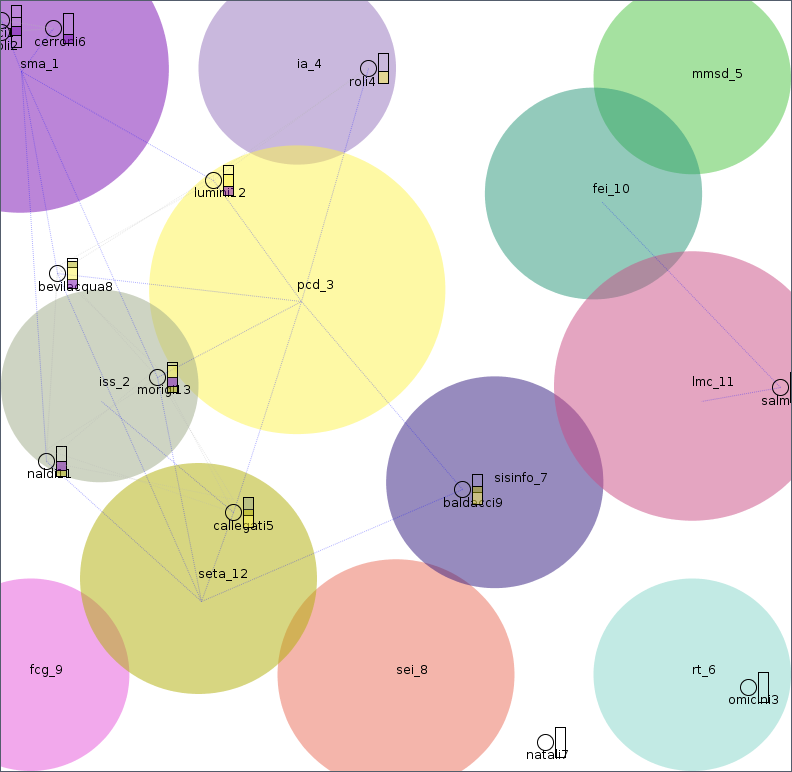
\includegraphics[width=13cm]{./imgs/screen1.png}
  \caption{Screenshot 1}
  \label{fig:screens1}
\end{figure}

\begin{figure}[!h]
  \centering
  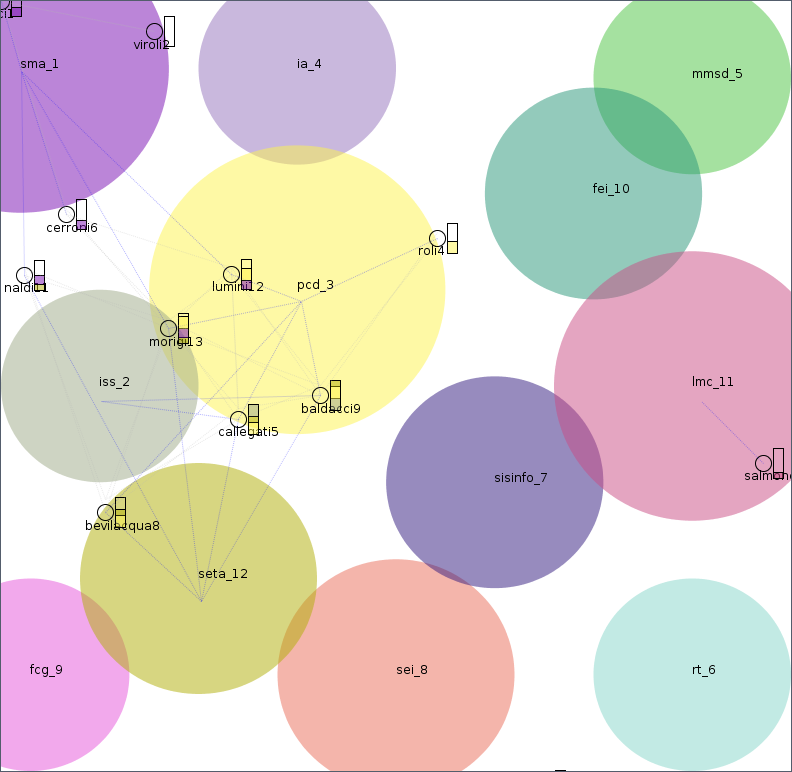
\includegraphics[width=13cm]{./imgs/screen2.png}
  \caption{Screenshot 2}
  \label{fig:screens2}
\end{figure}

\begin{figure}[!h]
  \centering
  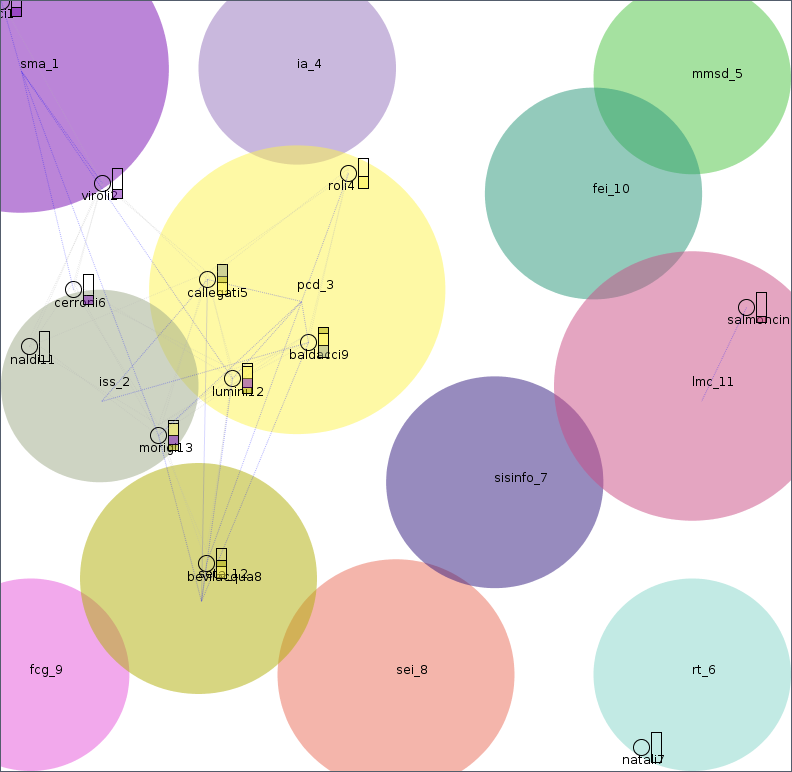
\includegraphics[width=13cm]{./imgs/screen3.png}
  \caption{Screenshot 3}
  \label{fig:screens3}
\end{figure}

\begin{figure}[!h]
  \centering
  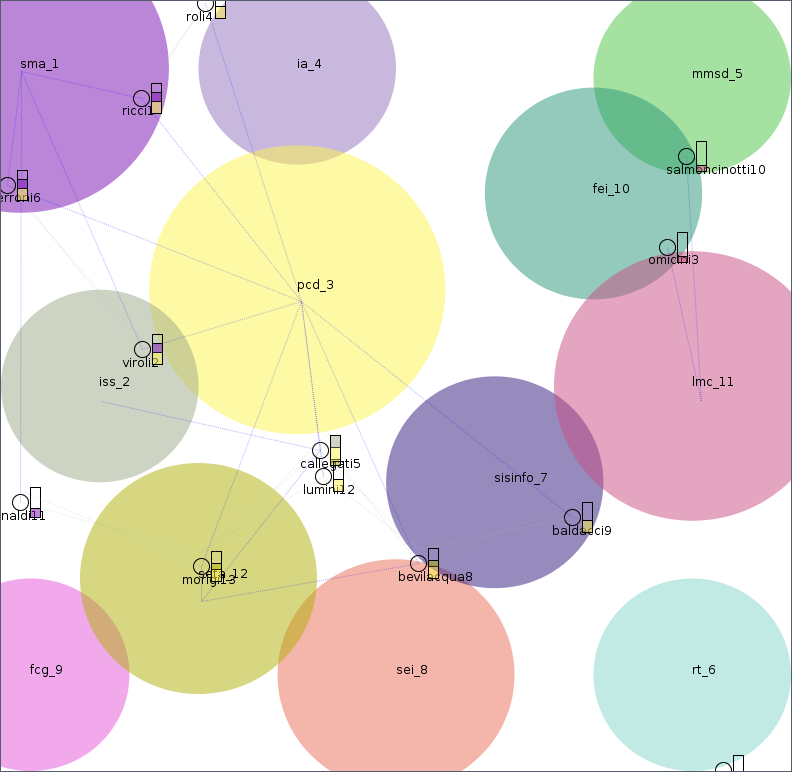
\includegraphics[width=13cm]{./imgs/screen4.png}
  \caption{Screenshot 4}
  \label{fig:screens4}
\end{figure}

\FloatBarrier

%\section{Theoretical background}

\subsection{Hovering Information System}

The hovering information system is composed by two main components: mobile
nodes and pieces of hovering information.

\emph{Mobile nodes} are components moving into the environment with a limited
communication range, capable of communicate to peers, discover neighbors,
access and store (into a limited buffer) pieces of
hovering information. A mobile node is assumed able to determinate its
geographic position, speed and direction.

\emph{Pieces of hovering information} are data that have to \emph{survive}
inside a circular area centered at a location called \emph{anchor location} and
having a radius called \emph{anchor radius}. The survivability goal of a piece
of hovering information is achieved moving or replicating the piece itself
through the mobile nodes. A piece of hovering information may have some
policies controlling the movement between nodes.

In an hovering information system, three main requirements may be defined for each
piece of hovering information \cite{hover}:
\begin{description}
	\item[Survivability:] a piece of hovering information is alive at some time
		$t$, if there is at leas one node hosting a replica of this information.
		\\
		$survivability = \frac{alive\_time}{total\_time}$
	\item[Availability:] a piece of hovering information is available at some time
		$t$, if there is at least one node in its anchor area hosting a replica of
		this information.
		\\
		$avaiability = \frac{avaiable\_time}{total\_time}$
	\item[Accessibility:] a piece of hovering information is accessible by a node
		at some time $t$, if the node is able to get this information; therefore, a
		replica exists in the node communication range.
		\\
		$accessibility = \frac{replica\_covered\_area}{anchor\_area}$
\end{description}



\bibliographystyle{plain}
%\nocite{*}
\bibliography{bib/bib,bib/implementation}{}

\end{document}
